\chapter{Introduction}

\begin{framed}
    \begin{itemize}
        \item Short history of SC (from Onnes to BCS)
        \item The discovery of LBCO and a brief overview of unconventional superconductivty
        \item Cuprates and competing orders (the possibility of many near-degenerate orders motivates this thesis)
        \item Microscopic vs Macroscopic (motivates the use of spectroscopic methods)
        \item Dopants (LSCO, LCO+O, LSCO+O, LNSCO, LBCO)
        \item Phase diagram (Tc, Tn, T* - macro stuff). How things are measured. Specific heat, Magnetization etc.
        \item Stripe order (why do we think it is important?). 
        \item Phase diagram including microscopic measurements (such as Kofu's).
        \item Other microscopic measured phenomena (I can only think of loop currents, others?)
        \item Theories (PDW, RVB, Loop currents, spin-fluctuation mediated SC). Are these even the same level of theory?
        \item Structural aspects of LSCO (The LTT problem, LBCO, LNSCO, define Q1 Q2, Superstripes). This should feed right into the motivation of the thesis.
        \item The relationship between ordering (such as stripes) and electronic band structure (from ARPES etc).
    \end{itemize}
\end{framed}

In this thesis, we explore certain aspects of the so-called high-temperature superconductors. While these materials were discovered fairly recently (1985), they have a rich history with hundreds of thousands of citations and, to this day, a lively debate surrounding the microscopic nature of this mysterious macroscopic quantum state. The purpose of this chapter is to briefly state the `the story so far' in broad strokes, and then dive deeper into state-of-the-art research relevant for the work performed in this thesis. 

\section{Superconductivity}
Superconductivity is a state of matter where a material is able to conduct electricity with \emph{zero} resistance below a certain critical temperature $T_\text{c}$. Since we, fortunately, live in a world where the `spherical cow in a vacuum' model does not apply, it is remarkable to find \emph{real} materials where electrons can propagate without friction. In fact, experiments have shown, that under the right conditions it is possible to keep a persistent superconducting current running for 100000 years [XX Phys. Rev. Lett. 10, 93]!

Superconductivity was first discovered in 1911 by Kamerlingh Onnes [XX], essentially as a consequence of being able to liquefy helium in 1908 [XX] and reach temperatures close to absolute zero. His low-temperature measurement of lead revealed a sudden drop in resistivity at \SI{4.2}{\kelvin}, as seen in the historic plot on figure \ref{fig:onnes}

\begin{figure}[]
    \centering
    \missingfigure{Onnes picture + Resisitivity plot}
    \caption{\textbf{Left}: Kammerling Onnes and his chief engineer in their cryogenics lab. \textbf{Right}: Resistivity as a function of temperature in elemental Lead.}
    \label{fig:onnes}
\end{figure}

Despite this remarkable experimental result, it would be 20 years for the next major milestone to appear. In 1933 the Meissner effect was discovered [XX], showing that superconducting materials would completely resist applied magnetic field by exhibiting perfect diamagnetism as shown in figure [XX]. In 1935 this effect was phenomenologically explained by the London equations [XX], showing that the Meissner effect is due to superconducting currents on the surface of the material. From their relatively simple set of equations, an observable length scale known as the penetration depth was defined
%
\[ \lambda = \sqrt{\frac{m}{\mu_0 n_s e^2}} \, \]
%
where $mu_0$ is the permeability of the material, $n_s$ the superconducting current, $m$ the mass and $e$ the electron charge\todo{check this}. This describes how an external magnetic field penetrates the superconductor through the relationship $B(x) = B(0) \exp (-x / \lambda)$. 

Another roughly 20 years would pass until Landaus work on phase transitions paved the way to understanding the superconducting phase transition as a thermodynamic quantity through the Ginzburg-Landau equations. This description predicts an additional characteristic length scale of the superconductor called the \emph{coherence length} and recasts the penetration depth. The ratio of these parameters, $\kappa$, were used to classify superconductors into type-I and type-II. Later on, in 19XX, XX used Ginzburg-Landau theory (GL theory) to explain the observation of a vortex lattice in thin-film type-II superconductors [XX], confidently proving the applicability of these principles. GL theory is a remarkable achievement that provides, as far as we know, a macroscopic description of superconductivity for \emph{all} known superconductors [XX].

Despite the descriptive power of GL theory, we are left with no recipe on how to construct, even theoretically, `better' superconductors. In order to manipulate material properties, it is necessary to understand the microscopic properties that lead to macroscopic behavior (e.g. how phonons influence thermal properties or how magnetic exchange influence magnetic properties. Inspired by GL theory, rapid progress towards a microscopic theory was being made in the mid 1950s, culminating in the famous BCS theory formulated by Bardeen, Cooper and Schrieffer [XX]. BCS theory is based on the assumption that an attractive interaction between electrons at the Fermi level can result in so-called `cooper-pairs', a bosonic quasi-particle consisting of an electron pair. The bosonic nature of this quasi-particle can, at low temperatures, result in a Bose-Einstein condensate where a large fraction of these electron pairs occupy the lowest energy quantum state.

This microscopic theory of superconductivity is supported a band gap at the Fermi level (where the cooper pairs form), the critical behaviour of this band gap as one approaches $T_\text{c}$ [XX] and the exponential behavior of the heat capacity in Vanadium near $T_\text{c}$ [XX]\todo{perhaps some data}. While BCS theory predicts an attractive interaction between electrons, there is no assumption on the nature of this interaction in the original description. A couple of experiments performed a few years prior showed that $T_\text{c}$ of Hg$^{198}$ was higher when compared to that of natural Hg (avg. atomic weight of 200.6). Since the chemistry of these materials can be assumed identical, this experiment suggests a positive correlation between phonon frequencies and $T_\text{c}$, since lighter elements vibrate faster. With this result, BCS theory could relate the attractive interaction to phonon frequencies and predict a relative relationship between isotopic mass and critical temperature:
%
\[ T_\text{c} \propto \frac{1}{\sqrt{m_\text{ion}}} \]
%
With BCS theory, superconductivity in many elemental metals were essentially `solved' with the identification of phonon-mediated superconductivity. Unfortunately, this discovery also set a \emph{practical} upper limit on $T_\text{c}$. In order to increase phonon frequencies, and critical temperatures, we need materials with low mass atomic species, while still being crystalline. ambient pressure this practical upper limit is often quoted to be around \SI{30}{\kelvin} [XX]. A good demonstration of this principle is actually a counter-example where researchers were able to reach a critical temperature of $T_\text{c} = \SI{200}{\kelvin}$ by applying a pressure of \SI{155}{\giga\pascal} to H$_2$S. This material contains the light atomic species we require, but cannot crysallize at ambient pressures so we can only reach high critical temperatures under extreme conditions.

While this thesis has nothing to do with BCS superconductors and, in principle, could have been written without ever mentioning them, I believe that the history of conventional superconductivity emphazises exactly what is desired from a `solution' to high-temperature superconductivity. It is also a fascinating story due to the fact that the tools to solve the problem were not even close to being developed when the phenomenon was discovered. It took roughly 50 years for a satisfying conclusion and we have only been working on the cuprates for roughly 30 years. As experimentalists we hope that our explorations can lead to discoveries such as the one in figure [XX: isotopic mass]. 

\section{Cuprates}
Roughly 30 years after BSC theory, in 1986, Bednorz and Muller discovered a new type of superconductor while trying to manupulate the Jahn-Teller effect by hole doping La$_2$CuO$_4$. While their efforts were successful\todo{were they? it certainly exists in LBCO}, these experiments had the remarkable side effect of creating the highest-$T_\text{c}$ superconductor at the time. Very shortly after in 19XX, the sister-compound YBCO was discovered, shattering previous records and finally achiving a critical temperature $T_\text{c} = \SI{110}{\kelvin}$ that could be reached using liquid nitrogen. 

While the increased critical temperatures are remarkable on their own, it quickly bacame apparent that we were dealing with a completely new type of superconductivty which cannot be explained with BCS theory. It was quickly realized that the normal state ($T > T_\text{c}$) of cuprate superconductors is as, if not more, complex when compared to the superconducting state. The BCS assumption of being metallic in the normal state is thus not fulfilled. In addition, no simple relationship between isotopic mass and $T_\text{c}$ has been found (see e.g. [XX: LESCO LNSCO paper]).

A general phase diagram for this family of cuprate is shown in figure \ref{fig:cuprate_phase_keimer} and a selction of materials from the cuprate `family' is shown in figure \ref{fig:cuprate_family_structures}. A quick glance at figure \ref{fig:cuprate_family_structures} reveals that they are all characterized by one or more layers with copper on a square lattice seperated by oxygen atoms. These copper-oxide layers are seperated by [XX what should I call this]. 

\begin{figure}
    \centering
    \missingfigure{cuprate phase diagram by keimer}
    \caption[cuprate phase diagram: keimer]{cuprate phase diagram: keimer}
    \label{fig:cuprate_phase_keimer}
\end{figure}

\begin{figure}
    \centering
    \missingfigure{selection of cuprate crystal structures}
    \caption[various cuprate structures]{various cuprate structures}
    \label{fig:cuprate_family_structures}
\end{figure}

By substitution, introduction or removal of certain atomic species we can effectively remove electrons from the system in a process known as hole-doping. As shown in figure \ref{fig:cuprate_phase_keimer}, cuprates are only superconducting for a narrow range of hole doping typically between $n_h = 0.05$ and $n_h = 0.25$ with a maximum around $n_h = 0.15$. This region is known as the `superconducting dome'. I emphasize here the very different states of matter at the boundaries of this dome; over-doped cuprates are typically metals while underdoped cuprates are magnetic insulators. In some sense, superconductivity occurs in a region between localized (magnet) and itenerant (metal) behvaiour.


\section{LSCO}

In this section, we look more closely at a specific family cuprates derived from La$_2$CuO$_4$, relevant to this thesis. Since one has to be careful about extrapolating conclusions based on specific samples to unconventional superconductivity as a whole, I will attempt to provide the broader context when applicable. While this chapter will primarily survey experiments and theories relevant to the work performed in this thesis, I emphasize the almost unmanageable amount of novel phenomena discovered in these compounds. It is my strong belief that `solving' the cuprates will require clues from many areas of research and it is my intention to highlight some of these clues here, even when outside the scope of this thesis.

\begin{figure}
    \centering
    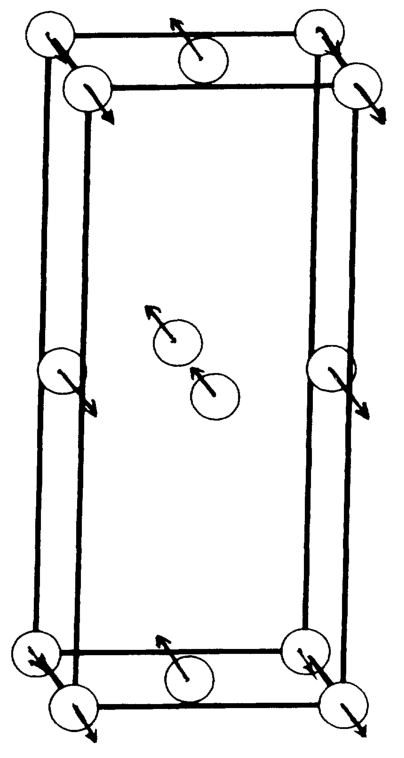
\includegraphics[width=0.5\textwidth]{fig/lsco/lsco_afm.png}
    \caption[AFM structure of LSCO]{AFM structure of LSCO}
    \label{fig:lsco_afm}
\end{figure}

\section{LSCO+O}